\documentclass[11pt,a4paper]{report}
\usepackage[textwidth=37em,vmargin=30mm]{geometry}
\usepackage{calc,xunicode,amsmath,amssymb,paralist,enumitem,tabu,booktabs,datetime2,xeCJK,xeCJKfntef,listings}
\usepackage{tocloft,fancyhdr,tcolorbox,xcolor,graphicx,eso-pic,xltxtra,xelatexemoji}

\newcommand{\envyear}[0]{2024}
\newcommand{\envdatestr}[0]{2024-11-08}
\newcommand{\envfinaldir}[0]{webdb/2024/20241108/final}

\usepackage[hidelinks]{hyperref}
\hypersetup{
    colorlinks=false,
    pdfpagemode=FullScreen,
    pdftitle={Web Digest - \envdatestr}
}

\setlength{\cftbeforechapskip}{10pt}
\renewcommand{\cftchapfont}{\rmfamily\bfseries\large\raggedright}
\setlength{\cftbeforesecskip}{2pt}
\renewcommand{\cftsecfont}{\sffamily\small\raggedright}

\setdefaultleftmargin{2em}{2em}{1em}{1em}{1em}{1em}

\usepackage{xeCJK,xeCJKfntef}
\xeCJKsetup{PunctStyle=plain,RubberPunctSkip=false,CJKglue=\strut\hskip 0pt plus 0.1em minus 0.05em,CJKecglue=\strut\hskip 0.22em plus 0.2em}
\XeTeXlinebreaklocale "zh"
\XeTeXlinebreakskip = 0pt


\setmainfont{Brygada 1918}
\setromanfont{Brygada 1918}
\setsansfont{IBM Plex Sans}
\setmonofont{JetBrains Mono NL}
\setCJKmainfont{Noto Serif CJK SC}
\setCJKromanfont{Noto Serif CJK SC}
\setCJKsansfont{Noto Sans CJK SC}
\setCJKmonofont{Noto Sans CJK SC}

\setlength{\parindent}{0pt}
\setlength{\parskip}{8pt}
\linespread{1.15}

\lstset{
	basicstyle=\ttfamily\footnotesize,
	numbersep=5pt,
	backgroundcolor=\color{black!5},
	showspaces=false,
	showstringspaces=false,
	showtabs=false,
	tabsize=2,
	captionpos=b,
	breaklines=true,
	breakatwhitespace=true,
	breakautoindent=true,
	linewidth=\textwidth
}






\newcommand{\coverpic}[2]{
    % argv: itemurl, authorname
    Cover photo by #2~~(\href{#1}{#1})
}
\newcommand{\makeheader}[0]{
    \begin{titlepage}
        % \newgeometry{hmargin=15mm,tmargin=21mm,bmargin=12mm}
        \begin{center}
            
            \rmfamily\scshape
            \fontspec{BaskervilleF}
            \fontspec{Old Standard}
            \fontsize{59pt}{70pt}\selectfont
            WEB\hfill DIGEST
            
            \vfill
            % \vskip 30pt
            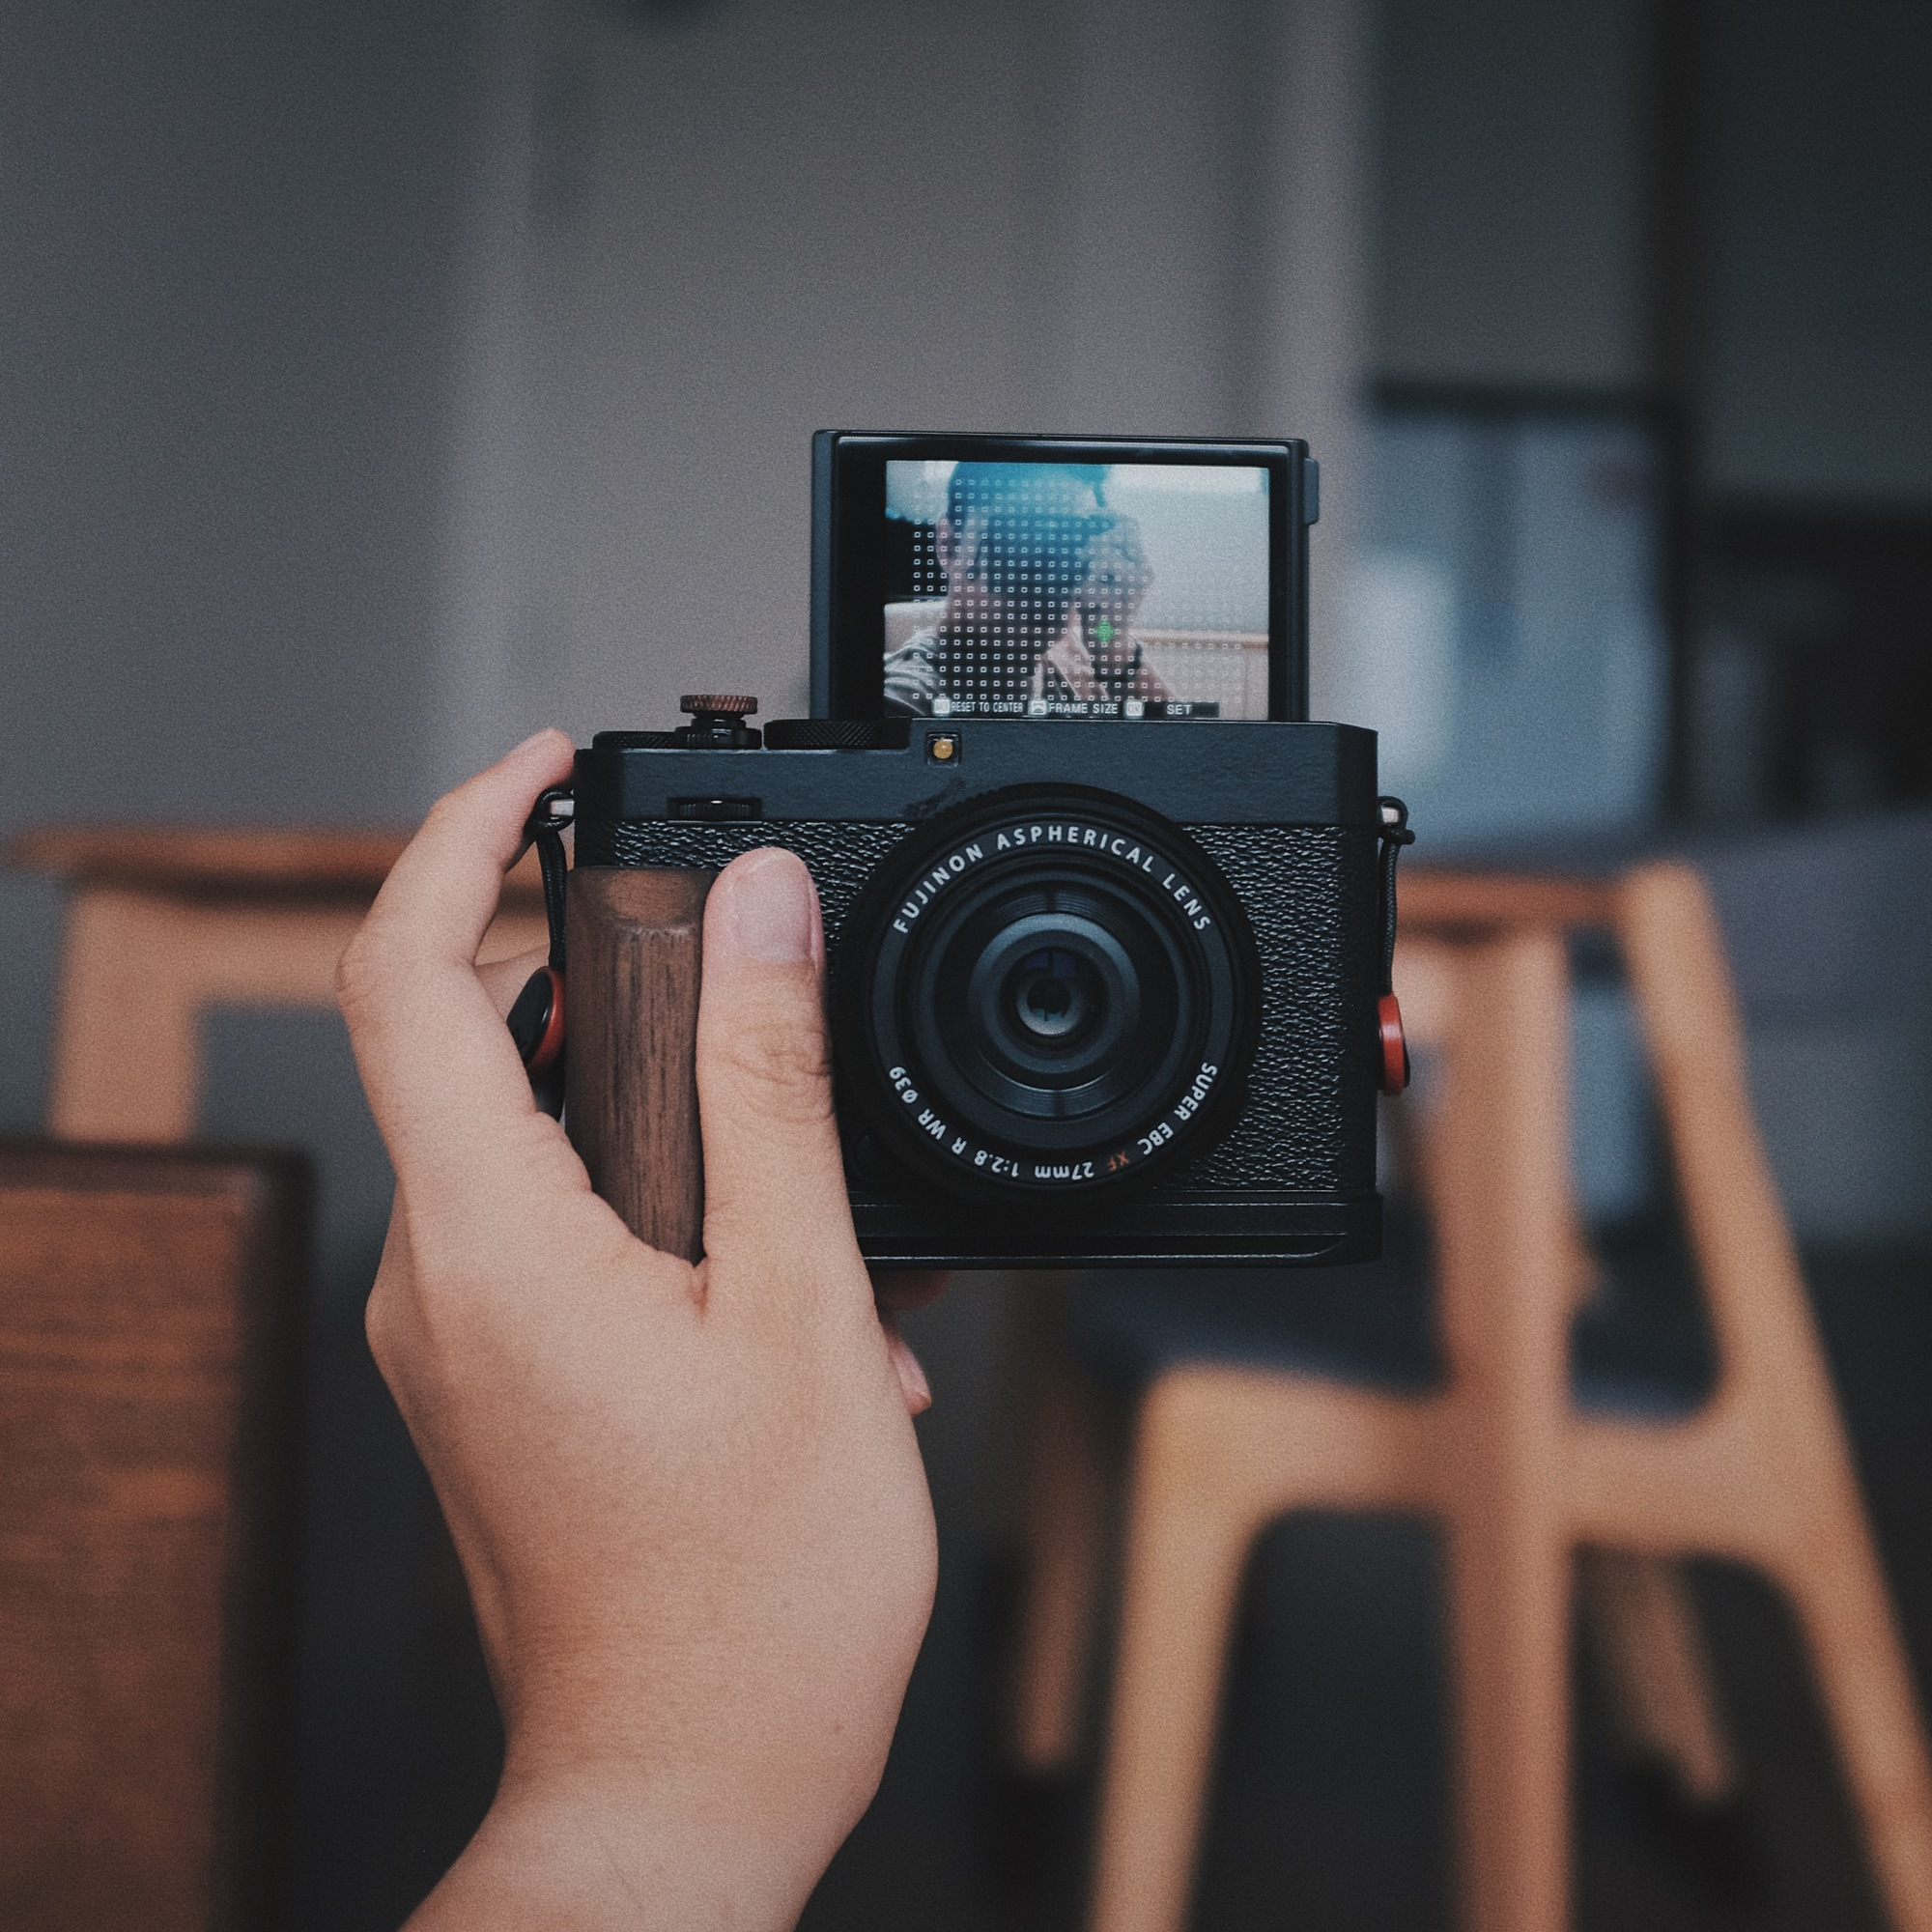
\includegraphics[width=\linewidth]{\envfinaldir/coverpic-prod.jpg}\par
            % \vskip 30pt
            \vfill

            \normalsize\rmfamily\scshape
            \copyright{} The Web Digest Project \hfill\large \envdatestr
        \end{center}
    \end{titlepage}
    % \restoregeometry
}
\newcommand{\simplehref}[1]{%
    \textcolor{blue!80!green}{\href{#1}{#1}}%
}
\renewcommand{\contentsname}{\center\Huge\sffamily\bfseries Contents\par\vskip 20pt}
\newcounter{ipartcounter}
\setcounter{ipartcounter}{0}
\newcommand{\ipart}[1]{
    % \vskip 20pt
    \clearpage
    \stepcounter{ipartcounter}
    \phantomsection
    \addcontentsline{toc}{chapter}{#1}
    % \begin{center}
    %     \Huge
    %     \sffamily\bfseries
    %     #1
    % \end{center}
    % \vskip 20pt plus 7pt
}
\newcounter{ichaptercounter}
\setcounter{ichaptercounter}{0}
\newcommand{\ichapter}[1]{
    % \vskip 20pt
    \clearpage
    \stepcounter{ichaptercounter}
    \phantomsection
    \addcontentsline{toc}{section}{\numberline{\arabic{ichaptercounter}}#1}
    \begin{center}
        \Huge
        \sffamily\bfseries
        #1
    \end{center}
    \vskip 20pt plus 7pt
}
\newcommand{\entrytitlefont}[1]{\subsection*{\raggedright\Large\sffamily\bfseries#1}}
\newcommand{\entryitemGeneric}[2]{
    % argv: title, url
    \parbox{\linewidth}{
        \entrytitlefont{#1}\par\vskip 5pt
        \footnotesize\ttfamily\mdseries
        \simplehref{#2}
    }\vskip 11pt plus 11pt minus 1pt
}
\newcommand{\entryitemGithub}[3]{
    % argv: title, url, desc
    \parbox{\linewidth}{
        \entrytitlefont{#1}\par\vskip 5pt
        \footnotesize\ttfamily\mdseries
        \simplehref{#2}\par\vskip 5pt
        \small\rmfamily\mdseries#3
    }\vskip 11pt plus 11pt minus 1pt
}
\newcommand{\entryitemAp}[3]{
    % argv: title, url, desc
    \parbox{\linewidth}{
        \entrytitlefont{#1}\par\vskip 5pt
        \footnotesize\ttfamily\mdseries
        \simplehref{#2}\par\vskip 5pt
        \small\rmfamily\mdseries#3
    }\vskip 11pt plus 11pt minus 1pt
}
\newcommand{\entryitemHackernews}[3]{
    % argv: title, hnurl, rawurl
    % \parbox{\linewidth}{
    %     \entrytitlefont{#1}\par\vskip 5pt
    %     \footnotesize\ttfamily\mdseries
    %     \simplehref{#3}\par
    %     \textcolor{black!50}{\href{#2}{#2}}
    % }\vskip 11pt plus 11pt minus 1pt
    \begin{minipage}{\linewidth}
            \entrytitlefont{#1}\par\vskip 5pt
            \footnotesize\ttfamily\mdseries
            \simplehref{#3}\par
            \textcolor{black!50}{\href{#2}{#2}}
    \end{minipage}\par\vskip 11pt plus 11pt minus 1pt
}







\begin{document}

\makeheader

\tableofcontents\clearpage




\ipart{Developers}
\ichapter{Hacker News}
\entryitemTwoLinks{Kagi Translate}{https://news.ycombinator.com/item?id=42080012}{https://blog.kagi.com/kagi-translate}

\entryitemTwoLinks{Ask HN: Life-changing purchases since 2020? (Under \$100 and under \$1000)}{https://news.ycombinator.com/item?id=42079768}{https://news.ycombinator.com/item?id=42079768}

\entryitemTwoLinks{QNX is now free for anything non-commercial, plus there's an RPi image}{https://news.ycombinator.com/item?id=42079460}{https://blackberry.qnx.com/en/products/qnx-everywhere}

\entryitemTwoLinks{Mushroom Color Atlas}{https://news.ycombinator.com/item?id=42078581}{https://www.mushroomcoloratlas.com/}

\entryitemTwoLinks{Launch HN: Codebuff (YC F24) – CLI tool that writes code for you}{https://news.ycombinator.com/item?id=42078536}{https://news.ycombinator.com/item?id=42078536}

\entryitemTwoLinks{Google banned me from Google Voice}{https://news.ycombinator.com/item?id=42078324}{https://www.dannyguo.com/blog/google-banned-me-from-google-voice}

\entryitemTwoLinks{Show HN: BemiDB – Postgres read replica optimized for analytics}{https://news.ycombinator.com/item?id=42078067}{https://github.com/BemiHQ/BemiDB}

\entryitemTwoLinks{Richard A. Cash, who saved millions from dehydration, has died}{https://news.ycombinator.com/item?id=42077735}{https://www.nytimes.com/2024/11/02/science/richard-cash-dead.html}

\entryitemTwoLinks{AI for real-time fusion plasma behavior prediction and manipulation}{https://news.ycombinator.com/item?id=42077319}{https://control.princeton.edu/machine-learning-for-rt-profile-control-in-tokamaks/}

\entryitemTwoLinks{Using Ghidra and Python to reverse engineer Ecco the Dolphin}{https://news.ycombinator.com/item?id=42076884}{https://32bits.substack.com/p/under-the-microscope-ecco-the-dolphin}

\entryitemTwoLinks{XMPP: The Gem of Instant Messaging}{https://news.ycombinator.com/item?id=42076814}{https://adele.pages.casa/md/blog/xmpp-the-forgotten-gem-of-instant-messaging.md}

\entryitemTwoLinks{Sixteen U.S. states still ban community-owned broadband networks}{https://news.ycombinator.com/item?id=42076719}{https://www.techdirt.com/2024/11/07/16-u-s-states-still-ban-community-owned-broadband-networks-because-att-and-comcast-told-them-to/}

\entryitemTwoLinks{Excerpts from a conversation about personal information management}{https://news.ycombinator.com/item?id=42076200}{https://sachachua.com/blog/2024/11/excerpts-from-a-conversation-with-john-wiegley-johnw-and-adam-porter-alphapapa-about-personal-information-management/}

\entryitemTwoLinks{Accelerating the Performance of Rosetta in Linux VMs on Apple Silicon}{https://news.ycombinator.com/item?id=42074592}{https://developer.apple.com/documentation/virtualization/accelerating\_the\_performance\_of\_rosetta}

\entryitemTwoLinks{Even Microsoft Notepad is getting AI text editing now}{https://news.ycombinator.com/item?id=42074083}{https://www.theverge.com/2024/11/6/24289707/microsoft-notepad-ai-text-editing-rewrite}

\entryitemTwoLinks{Evaluating the world model implicit in a generative model}{https://news.ycombinator.com/item?id=42073801}{https://arxiv.org/abs/2406.03689}

\entryitemTwoLinks{Nvidia Rides AI Wave to Pass Apple as Largest Company}{https://news.ycombinator.com/item?id=42073066}{https://www.bloomberg.com/news/articles/2024-11-05/nvidia-rides-ai-wave-to-pass-apple-as-world-s-largest-company}

\entryitemTwoLinks{I'm not mutable, I'm partially instantiated}{https://news.ycombinator.com/item?id=42073001}{https://blog.dnmfarrell.com/post/incomplete-data-structures/}

\entryitemTwoLinks{The English Paradox: Four decades of life and language in Japan}{https://news.ycombinator.com/item?id=42072647}{https://www.tokyodev.com/articles/the-english-paradox-four-decades-of-life-and-language-in-japan}

\entryitemTwoLinks{Australia proposes ban on social media for those under 16}{https://news.ycombinator.com/item?id=42071310}{https://www.reuters.com/technology/cybersecurity/australia-proposes-ban-social-media-those-under-16-2024-11-06/}\ichapter{Phoronix}
\entryitemGeneric{\hskip 0pt{}NVIDIA GH200 Grace CPU vs. AMD EPYC 9005 Turin CPU Performance}{https://www.phoronix.com/review/nvidia-grace-epyc-turin}

\entryitemGeneric{\hskip 0pt{}Linux 6.13 To Allow Controlling Zero RPM Feature For Radeon RX 7000 Series GPUs}{https://www.phoronix.com/news/Linux-6.13-AMDGPU-Zero-Fan}

\entryitemGeneric{\hskip 0pt{}FreeBSD Reduces OS Support From 5 To 4 Years, Continues Collaboration With AMD}{https://www.phoronix.com/news/FreeBSD-2024-Q3-Report}

\entryitemGeneric{\hskip 0pt{}Mesa RADV Driver Delivers Conformant Vulkan 1.3 Support For Old AMD GFX6/GFX7 GPUs}{https://www.phoronix.com/news/RADV-GFX6-GFX7-Vulkan-1.3}

\entryitemGeneric{\hskip 0pt{}Haiku Enjoyed A Busy October Implementing More Features}{https://www.phoronix.com/news/Haiku-OS-October-2024}

\entryitemGeneric{\hskip 0pt{}Mesa 24.3 Merges Vulkan FIFO Support On Wayland}{https://www.phoronix.com/news/Mesa-24.3-Vulkan-FIFO}

\entryitemGeneric{\hskip 0pt{}OpenCL Headers \& SDK Updated For OpenCL 3.0.17}{https://www.phoronix.com/news/OpenCL-3.0.17-Headers-SDK}

\entryitemGeneric{\hskip 0pt{}AMD ROCm 6.2.4 Released With Radeon PRO V710 Support \& Documentation Updates}{https://www.phoronix.com/news/AMD-ROCm-6.2.4-Released}

\entryitemGeneric{\hskip 0pt{}GIMP 3.2 Will Aim To Be Out Within One Year Of GIMP 3.0}{https://www.phoronix.com/news/GIMP-3.2-One-Year-Goal}


\ipart{Developers~~~~(zh-Hans)}
\ichapter{Solidot}
\entryitemGeneric{\hskip 0pt{}Linux Man pages 维护者获得赞助恢复工作}{https://www.solidot.org/story?sid=79710}

\entryitemGeneric{\hskip 0pt{}法官裁决 Google 没有义务向礼品卡诈骗受害者退款}{https://www.solidot.org/story?sid=79709}

\entryitemGeneric{\hskip 0pt{}2024 年将是平均气温比工业化前水平高出 1.5 摄氏度的第一年}{https://www.solidot.org/story?sid=79708}

\entryitemGeneric{\hskip 0pt{}Windows 记事本引入生成式 AI 功能}{https://www.solidot.org/story?sid=79707}

\entryitemGeneric{\hskip 0pt{}失聪的雄蚊失去了交配的兴趣}{https://www.solidot.org/story?sid=79706}

\entryitemGeneric{\hskip 0pt{}GIMP 项目计划在 GIMP 3.0 正式发布一年内推出 3.2}{https://www.solidot.org/story?sid=79704}

\entryitemGeneric{\hskip 0pt{}澳大利亚提议禁止 16 岁以下儿童使用社交媒体}{https://www.solidot.org/story?sid=79703}

\entryitemGeneric{\hskip 0pt{}OpenAI 收购了域名 Chat.com}{https://www.solidot.org/story?sid=79702}

\entryitemGeneric{\hskip 0pt{}加拿大禁止 TikTok 在其境内运营}{https://www.solidot.org/story?sid=79701}

\entryitemGeneric{\hskip 0pt{}英特尔因 13-14 代酷睿 CPU 电压不稳问题被起诉}{https://www.solidot.org/story?sid=79700}

\entryitemGeneric{\hskip 0pt{}勒索组织要求法国施耐德公司用法棍支付赎金}{https://www.solidot.org/story?sid=79699}

\entryitemGeneric{\hskip 0pt{}下一代 Switch 将支持向后兼容}{https://www.solidot.org/story?sid=79698}

\entryitemGeneric{\hskip 0pt{}因无人维护 Linux 6.13 将移除 Fieldbus 子系统}{https://www.solidot.org/story?sid=79697}

\entryitemGeneric{\hskip 0pt{}猫脑的衰老与人类相似}{https://www.solidot.org/story?sid=79696}

\entryitemGeneric{\hskip 0pt{}早期黑洞吞噬物质速率超过理论上限的 40 倍}{https://www.solidot.org/story?sid=79695}

\entryitemGeneric{\hskip 0pt{}积极锻炼无法抵消久坐的不良后果}{https://www.solidot.org/story?sid=79694}

\entryitemGeneric{\hskip 0pt{}GIMP 3.0 RC1 开始测试}{https://www.solidot.org/story?sid=79693}

\entryitemGeneric{\hskip 0pt{}世界第一颗木制卫星发射升空}{https://www.solidot.org/story?sid=79692}

\entryitemGeneric{\hskip 0pt{}Google 收到了逾百亿 DMCA 删除请求}{https://www.solidot.org/story?sid=79691}

\entryitemGeneric{\hskip 0pt{}Mozilla 基金会裁员 30\%,关闭倡导和全球项目部门 }{https://www.solidot.org/story?sid=79690}\ichapter{V2EX}
\entryitemGeneric{\hskip 0pt{}[问与答] 国际版安卓手机购买的正确方式(香港/淘宝/转运?)}{https://www.v2ex.com/t/1087600}

\entryitemGeneric{\hskip 0pt{}[问与答] 主板不能开启内存 XMP 是什么原因吗?}{https://www.v2ex.com/t/1087599}

\entryitemGeneric{\hskip 0pt{}[程序员] 新的 M4 Mac Mini 各位搭配什么 [键盘+鼠标] ?或者 [键盘+触控板] 的体验怎么样?}{https://www.v2ex.com/t/1087598}

\entryitemGeneric{\hskip 0pt{}[Google] [help] downie 突然不能下载 youtube 视频了,大家有什么其他工具推荐么?}{https://www.v2ex.com/t/1087596}

\entryitemGeneric{\hskip 0pt{}[程序员] 读大佬们帖子,关于《独立开发/副业》深夜思考}{https://www.v2ex.com/t/1087595}

\entryitemGeneric{\hskip 0pt{}[硬件] 求笔记本电脑推荐 Linux or mac?}{https://www.v2ex.com/t/1087594}

\entryitemGeneric{\hskip 0pt{}[问与答] iPhone 用户推荐买小米手环 9pro 吗}{https://www.v2ex.com/t/1087593}

\entryitemGeneric{\hskip 0pt{}[Netflix] 看 netflix 怎么选中文字幕呢}{https://www.v2ex.com/t/1087592}

\entryitemGeneric{\hskip 0pt{}[问与答] vscode 有无让编辑窗口单独最大化的快捷键?}{https://www.v2ex.com/t/1087590}

\entryitemGeneric{\hskip 0pt{}[奇思妙想] 美国这国运不是一般的牛逼。}{https://www.v2ex.com/t/1087589}

\entryitemGeneric{\hskip 0pt{}[问与答] 现在还有可以查出开房记录的社工库吗?}{https://www.v2ex.com/t/1087588}

\entryitemGeneric{\hskip 0pt{}[分享创造] 我开发了一个 Chrome 浏览器插件: ShareTo,一站式的社交媒体分享解决方案}{https://www.v2ex.com/t/1087587}

\entryitemGeneric{\hskip 0pt{}[程序员] 做独立开发(副业)本质上是吃力不讨好投入产出比低的一件事情,不如学知识学技能}{https://www.v2ex.com/t/1087586}

\entryitemGeneric{\hskip 0pt{}[职场话题] 公司的项目太烂了,有点难以坚持下去了怎么办}{https://www.v2ex.com/t/1087585}

\entryitemGeneric{\hskip 0pt{}[分享创造] 为了学习英语常用表达,写了个笔记工具帮助自己学习}{https://www.v2ex.com/t/1087584}

\entryitemGeneric{\hskip 0pt{}[问与答] Tailscale 路由节点配置问题}{https://www.v2ex.com/t/1087582}

\entryitemGeneric{\hskip 0pt{}[问与答] 电动车(电自)加速和刹车时电机有飞机声是不是说明电机比较好?}{https://www.v2ex.com/t/1087581}

\entryitemGeneric{\hskip 0pt{}[互联网] 在微信搜了一下送水,刷抖音直接推桶装水直播}{https://www.v2ex.com/t/1087580}

\entryitemGeneric{\hskip 0pt{}[分享发现] 分享一个成本 60 元的远程 1080p50 帧 pikvm 的方案,流畅度吊打向日葵控控}{https://www.v2ex.com/t/1087579}

\entryitemGeneric{\hskip 0pt{}[问与答] 请教些 Mac 购买问题}{https://www.v2ex.com/t/1087578}

\entryitemGeneric{\hskip 0pt{}[问与答] 特效应该用 Framer Motion 吗}{https://www.v2ex.com/t/1087577}

\entryitemGeneric{\hskip 0pt{}[问与答] 求推荐图片转提示词的工具}{https://www.v2ex.com/t/1087576}

\entryitemGeneric{\hskip 0pt{}[酷工作] [上海][内推]米哈游社招,欢迎投递~}{https://www.v2ex.com/t/1087575}

\entryitemGeneric{\hskip 0pt{}[Kotlin] 我老人家翻译的 Kotlin 中文文档,正在更新到最新的 2.0.20 版}{https://www.v2ex.com/t/1087574}

\entryitemGeneric{\hskip 0pt{}[程序员] 电报机器人有这类开源的管理后台吗?}{https://www.v2ex.com/t/1087573}

\entryitemGeneric{\hskip 0pt{}[程序员] 做了一个"手动挡"的加密聊天应用,看看能不能给 v2er 当私信}{https://www.v2ex.com/t/1087572}

\entryitemGeneric{\hskip 0pt{}[宽带症候群] 大家快来,分享一下 clash 等客户端负载均衡的好方法吧}{https://www.v2ex.com/t/1087569}

\entryitemGeneric{\hskip 0pt{}[宽带症候群] 关于 ECH 的问题, cloudflare-ech.com 这个域名,走代理好还是直连好?}{https://www.v2ex.com/t/1087568}

\entryitemGeneric{\hskip 0pt{}[Apple] Apple Wallet (苹果钱包)已经保存的凭证(酒店会员卡)莫名其妙被吞}{https://www.v2ex.com/t/1087567}

\entryitemGeneric{\hskip 0pt{}[酷工作] [深圳] 高级项目技术经理}{https://www.v2ex.com/t/1087566}

\entryitemGeneric{\hskip 0pt{}[分享创造] 继续挨骂,继续努力。}{https://www.v2ex.com/t/1087565}

\entryitemGeneric{\hskip 0pt{}[iPhone] 我的 XR 无法开机了, 19 年 618 买的, 128G,没有维修过,估计是电池的问题,除了官网还有其他处理渠道吗?}{https://www.v2ex.com/t/1087564}

\entryitemGeneric{\hskip 0pt{}[生活] [记录]2024-11-07 夜晚加班}{https://www.v2ex.com/t/1087563}

\entryitemGeneric{\hskip 0pt{}[酷工作] Meshy 招聘啦! 全球顶级 3DAI 产品,正在招聘 AI Researcher/Graphics engineer /技术美术(技术向)}{https://www.v2ex.com/t/1087562}

\entryitemGeneric{\hskip 0pt{}[问与答] youtube 土耳其区要求更新付款方式了,有啥办法不?}{https://www.v2ex.com/t/1087561}

\entryitemGeneric{\hskip 0pt{}[反馈] 发帖吃 403+ban ip 是浏览器特征问题还是帖子内容问题?}{https://www.v2ex.com/t/1087558}

\entryitemGeneric{\hskip 0pt{}[分享发现] 微信 win PC 版 用 QT 重构了}{https://www.v2ex.com/t/1087555}

\entryitemGeneric{\hskip 0pt{}[微信] 微信穷封了吧?到处收 300 块!并且号还不通用??}{https://www.v2ex.com/t/1087554}

\entryitemGeneric{\hskip 0pt{}[Apple] AirPods Max 连接苹果设备和 Windows 设备的续航问题}{https://www.v2ex.com/t/1087553}

\entryitemGeneric{\hskip 0pt{}[职场话题] [Meshy] 全球 Top 3DAI 公司 Meshy 招聘啦!(AI Researcher、Graphics engineer、技术美术(技术向)等诸多岗位}{https://www.v2ex.com/t/1087552}

\entryitemGeneric{\hskip 0pt{}[Vim] 十分尴尬,被导师推荐去使用 JetBrains}{https://www.v2ex.com/t/1087551}

\entryitemGeneric{\hskip 0pt{}[问与答] 想学习 KVM 虚拟化技术}{https://www.v2ex.com/t/1087550}

\entryitemGeneric{\hskip 0pt{}[问与答] 各位大佬,谁是 PT 站 HDSKY 的注册会员,能否邀请下? 500M 电信宽带,nas 24h 运行}{https://www.v2ex.com/t/1087549}

\entryitemGeneric{\hskip 0pt{}[问与答] 搞不明白同花顺为什么可以从十一前的 100 涨到现在 330,东方财务才能够 10 涨到 30}{https://www.v2ex.com/t/1087544}

\entryitemGeneric{\hskip 0pt{}[OpenWrt] 求推荐 CPU 比较强的硬路由}{https://www.v2ex.com/t/1087543}

\entryitemGeneric{\hskip 0pt{}[程序员] 请问: 在 win10 上如何把本地 mysql 数据库转换为 postgresql 数据库}{https://www.v2ex.com/t/1087542}

\entryitemGeneric{\hskip 0pt{}[YouTube] YouTube Premium 土耳其地区 再次涨价了!}{https://www.v2ex.com/t/1087541}

\entryitemGeneric{\hskip 0pt{}[Apple] M1 Macbook Air 外接显示器有点发烫,有解吗?}{https://www.v2ex.com/t/1087540}

\entryitemGeneric{\hskip 0pt{}[分享创造] 我开发了一个 Chrome 浏览器插件: MarkdownIt,将任意网页内容导出为 Markdown 格式的文档}{https://www.v2ex.com/t/1087539}

\entryitemGeneric{\hskip 0pt{}[Google] 关于谷歌开发者身份认证?}{https://www.v2ex.com/t/1087538}


\ipart{Generic News}
\ichapter{AP News}
\entryitemWithDescription{\hskip 0pt{}A green giant: This year's 74-foot Rockefeller Center Christmas tree is en route from Massachusetts}{https://apnews.com/article/2abe2506f44a05949839561d98b442ce}{}

\entryitemWithDescription{\hskip 0pt{}Volunteer poll workers drown on a flood-washed highway in rural Missouri on Election Day}{https://apnews.com/article/acd757d8de6a6100af75ff26c6120770}{}

\entryitemWithDescription{\hskip 0pt{}Health care worker gets 2 years for accessing Ruth Bader Ginsburg's medical records}{https://apnews.com/article/b29394597228382d5514671f145c7e50}{}

\entryitemWithDescription{\hskip 0pt{}Canada orders TikTok's Canadian business to be dissolved but won't block app}{https://apnews.com/article/f290fed849bcdb26edb165d55b0aa225}{}

\entryitemWithDescription{\hskip 0pt{}Ten of thousands left without power as winter storm rolls over New Mexico and Colorado}{https://apnews.com/article/fa170e0561863ba4be415028f397b3e3}{}

\entryitemWithDescription{\hskip 0pt{}Indonesia's Mount Lewotobi Laki Laki erupts for the second time in a week}{https://apnews.com/article/3a3ca22d200412ebf869fd4dd1ea2b5d}{}

\entryitemWithDescription{\hskip 0pt{}Notre Dame marks arrival of Paris Olympics' iconic trackside bell as cathedral reopening nears}{https://apnews.com/article/22c181d4a67556e96378acc618d9adfe}{}

\entryitemWithDescription{\hskip 0pt{}In this Florida school district, some parents are pushing back against a cellphone ban}{https://apnews.com/article/89b0c8bdad325fb9a776f4384602a1a1}{}

\entryitemWithDescription{\hskip 0pt{}Japanese automaker Nissan cuts 9,000 jobs as its vehicles fail to sell}{https://apnews.com/article/b6fa5d02770a13908ecec11b6a9f8e8f}{}

\entryitemWithDescription{\hskip 0pt{}Australia plans a social media ban for children under 16}{https://apnews.com/article/e8259408c0b1456f41967decd474782a}{}

\entryitemWithDescription{\hskip 0pt{}Germany's coalition collapses dramatically. Scholz plans to lead with a minority government}{https://apnews.com/article/ca3ebd538bc0e71af272aa7f65b12c19}{}

\entryitemWithDescription{\hskip 0pt{}Deforestation in Brazil's Amazon drops by nearly 31\% compared to previous year}{https://apnews.com/article/4a8e25c3dee73ccd942677c192cf3e42}{}

\entryitemWithDescription{\hskip 0pt{}The first car made during Soviet-era in Poland goes on display 73 years later}{https://apnews.com/article/b821f6b848d2295dbb0c15c84027f326}{}\ichapter{Reuters}
\entryitemWithDescription{\hskip 0pt{}Trump allies push for Susie Wiles to be chief of staff}{https://www.reuters.com/world/us/trump-allies-push-susie-wiles-be-chief-staff-2024-11-07/}{Allies of President-elect Donald Trump are encouraging him to pick Susie Wiles, one of his two campaign managers, to be White House chief of staff as he prepares to start making personnel announcements in coming days, sources familiar...}

\entryitemWithDescription{\hskip 0pt{}Thousands under evacuation near Los Angeles as wildfire torches homes}{https://www.reuters.com/world/us/thousands-under-evacuation-orders-california-wildfires-destroy-homes-2024-11-07/}{Over ten thousand people were ordered to evacuate as fierce seasonal winds drove a wildfire down tinder-dry hillsides into ranches and...}

\entryitemWithDescription{\hskip 0pt{}Trump's team keen to unite anti-dictatorship exiles, Nicaragua dissident says}{https://www.reuters.com/world/americas/trumps-team-keen-unite-anti-dictatorship-exiles-nicaragua-dissident-says-2024-11-07/}{Members of U.S. President-elect Donald Trump\textquotesingle s transition team reached out to a leading Nicaraguan opposition figure on Thursday, saying they want to unite exiled communities from Nicaragua, Cuba, and Venezuela, the...}

\entryitemWithDescription{\hskip 0pt{}More families stream out of north Gaza, as tanks push deeper}{https://www.reuters.com/world/middle-east/more-families-stream-out-north-gaza-tanks-push-deeper-2024-11-07/}{Israeli forces ordered more evacuations, creating a fresh wave of displacement from northern...}

\entryitemWithDescription{\hskip 0pt{}Biden plans final Mideast peace push but will leaders ignore him?}{https://www.reuters.com/world/biden-plans-final-mideast-peace-push-will-leaders-ignore-him-2024-11-07/}{Donald Trump\textquotesingle s election may leave Washington without enough leverage to bend Israel and other regional players to its will before he becomes...}

\entryitemWithDescription{\hskip 0pt{}Nigeria rights body to present findings on abortion allegations against military}{https://www.reuters.com/world/africa/nigeria-rights-body-present-findings-abortion-allegations-against-military-2024-11-07/}{Nigeria\textquotesingle s human rights commission will on Friday deliver its findings from an investigation into Reuters reports, which found the military ran a secret, systematic and illegal abortion programme and massacred children in...}

\entryitemWithDescription{\hskip 0pt{}Plane brings 89 Russian nationals home from Lebanon, foreign ministry says}{https://www.reuters.com/world/plane-brings-89-russian-nationals-home-lebanon-foreign-ministry-says-2024-11-07/}{A Russian plane late on Thursday brought home 89 Russian nationals, including 34 children, evacuated from Lebanon, the foreign ministry...}

\entryitemWithDescription{\hskip 0pt{}Israel has made progress on assistance into Gaza but more needs to be done, Pentagon chief says}{https://www.reuters.com/world/middle-east/israel-has-made-progress-assistance-into-gaza-more-needs-be-done-pentagon-chief-2024-11-07/}{U.S. Defense Secretary Lloyd Austin said on Thursday that Israel had made some progress in getting assistance into Gaza but more needed to be...}

\entryitemWithDescription{\hskip 0pt{}13 people missing after fishing boat sinks in waters off South Korea, Yonhap reports}{https://www.reuters.com/world/asia-pacific/13-people-missing-after-fishing-boat-sinks-waters-off-south-korea-yonhap-reports-2024-11-07/}{A fishing boat has sunk in waters off South Korea\textquotesingle s Jeju Island with 14 sailors rescued and 13 missing, the Yonhap news agency reported on Friday citing the coast...}

\entryitemWithDescription{\hskip 0pt{}Putin praises Trump, says Russia is ready for dialogue}{https://www.reuters.com/world/putin-after-trump-win-says-struggle-new-world-order-is-underway-2024-11-07/}{Russian President Vladimir Putin on Thursday congratulated Donald Trump on winning the U.S. election, praised him for showing courage when a gunman tried to assassinate him, and said Moscow was ready for dialogue with the Republican...}

\entryitemWithDescription{\hskip 0pt{}Putin says Ukraine must remain neutral for there to be peace}{https://www.reuters.com/world/europe/putin-says-ukraine-must-remain-neutral-there-be-peace-2024-11-07/}{President Vladimir Putin said on Thursday that Ukraine should remain neutral for there to be a chance for peace, adding that the borders of Ukraine should be in accordance with the wishes of the people living in Russian-claimed...}

\entryitemWithDescription{\hskip 0pt{}Americans see immigration as top issue for Trump to tackle, Reuters/Ipsos poll finds}{https://www.reuters.com/world/americas/americans-see-immigration-top-issue-trump-tackle-reutersipsos-poll-finds-2024-11-07/}{Americans see immigration as the most pressing issue for President-elect Donald Trump to address, and a large majority believe he will order mass deportations of people living in the U.S. illegally, a Reuters/Ipsos poll that closed...}

\entryitemWithDescription{\hskip 0pt{}Zelenskiy says he is unaware of details of Trump plan to end war, bridles at ceasefire talk}{https://www.reuters.com/world/europe/zelenskiy-says-he-is-unaware-details-trump-plan-end-war-bridles-ceasefire-talk-2024-11-07/}{President Volodymyr Zelenskiy said on Thursday he was not aware of any details of U.S. President-elect Donald Trump\textquotesingle s plan to end the Ukraine war quickly and he was convinced a rapid end would entail major concessions for...}\ichapter{联合早报}
\entryitemWithDescription{沈泽玮:台湾冲突阻遏法案只叫不咬?}{https://www.zaobao.com/news/china/story20240918-4758889}{美国众议院9月9日开启了长达一星期的``中国周'',共通过25项主要涉华法案。(法新社) 美国众议院在当地时间9月9日开启了长达一星期的``中国周'',在美国总统和国会选举举行之前,密集表决数十项与中国有关的法案,共通过25项主要涉华法案……}

\entryitemWithDescription{欧盟电动车关税投票倒计时 中国在分歧中寻支持}{https://www.zaobao.com/news/china/story20240917-4758953}{欧盟27个成员国将于9月25日就是否继续对进口自中国的电动汽车额外征税进行最后表决。图为上海港等待装运出口的电动汽车。(彭博社) 欧盟对中国电动汽车加征关税的投票进入倒计时,正在欧洲访问的中国商务部部长王文涛与欧盟多国政府高层就此进行协商,试图在立场分歧的成员国中争取到更多支持。 受访学者研判,欧盟对中国电动汽车加征关税不可避免,但具体的加税方式和幅度仍有一定弹性,这是王文涛此行与各国谈判的重点……}

\entryitemWithDescription{港府今年将举办逾400项国庆活动}{https://www.zaobao.com/news/china/story20240917-4759341}{再过十多天就是中国国庆75周年,香港天星小轮展示``国庆75周年''\,``三天免费搭小轮''等标语迎国庆。(中新社) 再过十多天就是中国国庆75周年,香港特区政府今年将举办逾400项庆祝活动,希望通过一连串活动庆祝国庆,并且弘扬爱国主义教育及刺激消费。 港府星期二(9月17日)召开记者会,介绍各项庆祝国庆活动和特别优惠,涉及出行及吃喝玩乐等领域……}

\entryitemWithDescription{美空军部长:中国大陆军演精密化 为入侵封锁台湾做准备}{https://www.zaobao.com/news/china/story20240917-4759407}{美国空军部长肯德尔星期一(9月16日)在空军暨太空军协会的一场大会上致辞,提到中国对印太地区日益增长的威胁。(取自美国国防部网站) (华盛顿综合讯)美国空军部长肯德尔指,中国大陆军演的规模越来越大,也更加精密化,这是在专门为入侵、封锁台湾做准备。他也称,中国对印太地区的威胁现在已存在……}

\entryitemWithDescription{批准潜在对台备件军售案后 美派巡逻机过航台海}{https://www.zaobao.com/news/china/story20240917-4758770}{台军士兵8月26日在屏东县枋山训练场进行实弹演习时,从M1167 TOW运载车上发射一枚美制TOW-2A线导反坦克导弹。(路透社) (华盛顿/台北/北京综合讯)在批准潜在对台备件军售案之后,美国派遣反潜巡逻机过航台湾海峡,中国人民解放军东部战区则组织战机跟监美机,并誓言``坚决捍卫国家主权''……}

\entryitemWithDescription{李家超:若香港驻美经贸办被关 受害的是美企}{https://www.zaobao.com/news/china/story20240917-4758797}{香港特首李家超星期一(9月17日)警告,如果美国通过法案,导致香港驻美经贸办关闭,受害的是美国企业。图为李家超9月11日在``一带一路''高峰论坛上致辞。(彭博社) (香港综合讯)香港特首李家超警告,如果美国通过法案,导致香港驻美经贸办关闭,受害的是美国企业。 美国众议院上周通过《香港经济贸易办事处认证法案》,如果参议院也表决通过并交由总统签署成法,香港三个驻美国的经贸办可能将被强制关闭……}

\entryitemWithDescription{美国指中国航空工业集团员工企图实施黑客攻击}{https://www.zaobao.com/news/china/story20240917-4757988}{(华盛顿综合讯)中国航空航天巨头中国航空工业集团一名员工被指试图对美国宇航局、美国军方和其他目标展开黑客攻击。 据彭博社报道,美国检察官布坎南星期一(9月16日)在起诉书中,指控中国航空工业集团39岁的工程师吴宋(音译,Song Wu)企图从美国宇航局、空军、陆军和海军,以及联邦航空管理局取得电脑软件和源代码……}

\entryitemWithDescription{【东谈西论】恒大账务造假 普华永道是共犯还是被拖累?}{https://www.zaobao.com/news/china/story20240917-4756452}{因涉及恒大地产审计项目的违法行为,普华永道中国9月13日被中国财政部和证监会处以4.41亿人民币罚款并被令停业六个月, 广州分所被撤销……}

\entryitemWithDescription{戴庆成:香港输入人才计划大检阅}{https://www.zaobao.com/news/china/story20240917-4744978}{香港于2022年底推出高端人才通行证计划。(法新社) 2019年香港反修例风波过后,数以十万计港人移居海外,令香港出现人才荒。港府为了解决这个问题,在过去几年积极引入``新血'',当中以高才通计划最受瞩目,社会上也不时热议其成效。 高才通全称为高端人才通行证计划,于2022年底推出,申请人年收入须达到250万港元(约42万新元)以上,或本科毕业于全球百强大学并满足一定工作年限等……}

\entryitemWithDescription{中美希望稳定双边关系 中小国家可​​​搭建桥梁}{https://www.zaobao.com/news/china/story20240917-4745091}{中美元首去年11月在旧金山会晤后,双方都希望稳定两国关系,我国巡回大使陈庆珠认为,如果中美两国都认为走向战争不符合它们的利益,那么中小国家就可以做点什么,为双方搭建桥梁。 陈庆珠星期一(9月16日)在李光耀公共政策学院的一场研讨会上说,中国与西方的关系面对诸多困难,有中国智库表示,希望新加坡能协助在中美之间建立更多对话,``因为新加坡受美国信任,也在中国有渠道''……}

\entryitemWithDescription{陈庆珠:世界经历了三次``中国冲击'' 中美的主导力之争将继续}{https://www.zaobao.com/news/china/story20240917-4744996}{李光耀公共政策学院``思想之节庆''的一场研讨会,讨论``历史终结时的中国冲击''。左起是我国巡回大使陈庆珠、通商中国主席李奕贤、李光耀公共政策学院国际关系助理教授何莉菁、李光耀公共政策学院院长柯成兴……}

\entryitemWithDescription{上海遭遇75年来最强台风 扰乱民众中秋假期出行}{https://www.zaobao.com/news/china/story20240916-4745224}{台风贝碧嘉星期一(9月16日)登陆上海,维护人员星期一下午在衡山路上处理倒伏的树木。 (新华社) 台风造成上海上万株数目倒伏或折断。图为一棵倒下的大树砸坏一旁的建筑。(法新社) 台风贝碧嘉登陆上海后,黄浦江苏州河口潮位上涨,乌云密布。(中新社) 中国上海市星期一(9月16日)遭遇75年来最强台风``贝碧嘉''登陆,也是上海有记录以来首次有强台风侵袭……}

\entryitemWithDescription{陆男频长驱偷渡台湾在测试边防实力?}{https://www.zaobao.com/news/china/story20240916-4745161}{中国大陆一名王姓男子在中秋节前夕,乘橡皮艇从浙江宁波抵达台湾新北市林口,主动打电话投案,海巡署人员前去接他上岸。(自由時報) 中国大陆一名王姓男子划橡皮艇于上星期六清晨偷渡到台湾,隔天被新北市地方法院裁定羁押禁见。这是6月以来第二起大陆人士偷渡至台湾,此间专家质疑是否为海防破口,并怀疑对岸是否在测试台湾的边防实力……}

\entryitemWithDescription{中美时隔八月举行国防部工作会晤}{https://www.zaobao.com/news/china/story20240916-4745025}{(北京/华盛顿综合讯)中美双方上周末举行国防部工作会晤;美国官员称,美国积极进行美中两军外交活动,不代表美国对有关中国议题的处理方式发生任何改变。 据中国国防部星期天(15日)晚上通报,北京香山论坛结束后,第18次中美国防部工作会晤上星期六至星期天(9月14日至15日)在北京举行……}

\entryitemWithDescription{中国高校今年拟增足球运动本科专业}{https://www.zaobao.com/news/china/story20240916-4744925}{(北京综合讯)为了培养足球专业人才,中国大专学府今年度拟新增足球运动本科专业,以具体落实中国足球改革。 综合人民网和《南方都市报》报道,中国教育部上星期五(9月13日)发布《2024年度普通高等学校本科专业申报材料公示》。根据公示统计,今年度拟新增专业535个,涉及353所高校,其中39所高校新增足球运动专业……}

\entryitemWithDescription{香港23条首案 港男因穿``光时''上衣被定罪}{https://www.zaobao.com/news/china/story20240916-4743439}{(香港综合讯)香港一名无业男子,今年6月因穿印有2019年反修例抗争口号的上衣而被捕。他星期一承认违反煽动意图罪,成为在《维护国家安全条例》(即《香港基本法》第23条)下被定罪的第一人。 综合港媒《星岛日报》和路透社报道,27岁无业男子诸启邦今年6月12日在石门港铁站附近,未能出示身份证供查阅被警方拘捕……}

\entryitemWithDescription{美国务院:中国释放被关押近20年美籍牧师}{https://www.zaobao.com/news/china/story20240916-4744614}{(华盛顿综合电)中国释放被关押近20年的美国籍牧师,显示北京在中美关系的关键时刻展现善意。 综合彭博社、法新社和路透社报道,美国国务院发言人星期天(9月15日)说:``我们欢迎林大卫(音译,David Lin)从中华人民共和国的监狱获释。他已回返美国,这是他近20年来首次与家人见面。'' 林大卫的女儿艾丽斯告诉美国政治新闻网Politico,她的父亲将抵达得克萨斯州的圣安东尼奥……}

\entryitemWithDescription{中国驻泰使馆:近期并未向湄公河下游泄洪}{https://www.zaobao.com/news/china/story20240916-4743917}{(北京讯)泰国西北部的湄公河因洪水泛滥而决堤,中国否认这是中方泄洪所致,并称近来已持续减少云南景洪水电站的出库流量,以助下游地区抗洪。 中国驻泰国大使馆星期日(9月15日)深夜在官方微信公众号发文说,当天又有媒体报道称中国正在向湄公河泄洪,经向中国主管部门核实,使馆再次澄清,为帮助下游地区应对洪灾,中方近来持续稳定和减少景洪水电站出库流量,不可能对下游地区抗洪救灾形成压力……}

\entryitemWithDescription{加入美国储存可靠度评估计划 台湾军方编列预算采购三类型导弹}{https://www.zaobao.com/news/china/story20240916-4743826}{(台北讯)据台媒报道,台湾军方持续向美国采购可简易操作的导弹,预计在2024年、2031年以前获得400枚``标枪''反装甲导弹、2485枚``刺针''人携式防空导弹……}

\entryitemWithDescription{韩咏红:中美分头追逐全球南方}{https://www.zaobao.com/news/china/story20240916-4730719}{9月5日,中国外长王毅(中)同中非合作论坛非方现任共同主席国塞内加尔外长法勒(左)、下任共同主席国刚果外长加科索(右),在北京共同会见中外记者并答问。(路透社) 进入气候宜人的9月,中国接连举行了两场受瞩目的国际会议,一是聚集非洲53国国家元首与政要的中非合作论坛,接着是周末刚闭幕的北京香山论坛。 两场活动的参与者不同,规模也有很大差距……}

\entryitemWithDescription{菲律宾船只撤离中菲争议海域后 将再派船接替}{https://www.zaobao.com/news/china/story20240915-4730494}{这张在9月15日拍摄,并由菲律宾海岸警卫队提供的照片显示,菲律宾海岸警卫队船马格巴努亚号抵达了菲国巴拉望岛的一个港口。菲律宾早前以发现填海活动为由,今年4月派出马格巴努亚号前往萨比纳礁。(法新社/菲律宾海岸警卫队) 菲律宾国家海事委员会星期天(9月15日)发声明称,该国海岸警卫队一艘巡逻舰已离开萨比纳礁争议海域……}

\entryitemWithDescription{台风贝碧嘉直击中国华东 多趟本地与沪杭间航班取消}{https://www.zaobao.com/news/china/story20240915-4730611}{9月15日在上海外滩滨江步道上,一名外籍游客的雨伞被大风吹起。台风贝碧嘉的中心当天下午5时位于上海市东偏南方大约435公里的东海海面上,中心附近最大风力有13级。(中新社) (上海/新加坡综合讯)台风贝碧嘉预计将为中国华东沿海地区带来狂风暴雨,多趟往返新加坡与上海和杭州的航班取消……}






\clearpage
\leavevmode\vfill
\footnotesize

Copyright \copyright{} 2023-2024 Neruthes and other contributors.

This document is published with CC BY-NC-ND 4.0 license.

The entries listed in this newsletter may be copyrighted by their respective creators.

This newsletter is generated by the Web Digest project.

The newsletters are also delivered via Telegram channel \CJKunderline{\href{https://t.me/webdigestchannel}{https://t.me/webdigestchannel}}.\\
RSS feed is available at \CJKunderline{\href{https://webdigest.pages.dev/rss.xml}{https://webdigest.pages.dev/rss.xml}}.

This newsletter is available in PDF at
\CJKunderline{\href{https://webdigest.pages.dev/}{https://webdigest.pages.dev/}}.

The source code being used to generate this newsletter is available at\\
\CJKunderline{\href{https://github.com/neruthes/webdigest}{https://github.com/neruthes/webdigest}}.

This newsletter is also available in
\CJKunderline{\href{http://webdigest.pages.dev/readhtml/\envyear/WebDigest-20241108.html}{HTML}} and
\CJKunderline{\href{https://github.com/neruthes/webdigest/blob/master/markdown/\envyear/WebDigest-20241108.md}{Markdown}}.


\coverpic{https://unsplash.com/photos/a-close-up-of-a-plant-with-the-sun-in-the-background-dfkNxq-pUbg}{Maxim Tolchinskiy}


\end{document}
